
        We now want to investigate a larger class of differential equations.  These are the \boldgreen{partial differential equations} or PDEs.  These equations become yet more complicated to solve, but are very prevalent in the study of the physical world.
        
        Fundamentally, these are time-varying differential equations of vector and scalar fields of many variables.  The goal for us is to be able to recognize a few specific example equations and understand their behavior.  We will also be able to solve a few equations with our tools from studying ODE. However, it is easy to pose a PDE that is virtually impossible to solve.  
        
        \begin{df}{Partial Differential Equation}{pde}
        A \boldgreen{partial differential equation of a scalar field} of three spatial variables $x,y,z$ and a time variable $t$ is an expression of a scalar function $u(x,y,z,t)$, the partial derivatives of $u(x,y,z,t)$, and other functions.
        \end{df}
        
        \begin{df}{Vector Partial Differential Equation}{vec_pde}
        A \boldgreen{partial differential equation of a vector field}
        \[
        \vecfieldV(x,y,z,t) = \begin{bmatrix} V_1(x,y,z,t) \\ V_2(x,y,z,t) \\ V_3(x,y,z,t) \end{bmatrix}
        \]
        is an equation containing $\vecfieldV$, the (component) derivatives of $\vecfieldV$, and other vector fields.
        \end{df}
        
        With the difficulty of these expressions as is, we will concentrate solely on the equations with scalar functions.
    % %%%%%%%%%%%%%%%%%%%%%%%%%%%%%%%%%%%%%%%%%%%%%%%%%%%%%%%%%%%%%%%%%%%%%%%%%%%%%%%%%%%%
    % Examples of PDE
    % %%%%%%%%%%%%%%%%%%%%%%%%%%%%%%%%%%%%%%%%%%%%%%%%%%%%%%%%%%%%%%%%%%%%%%%%%%%%%%%%%%%%
    
        \section{Examples of PDE}
        
        \begin{ex}{Heat Equation}{heat_eqn}
        The \boldgreen{linear heat equation} in three dimensional space is the equation
        \[
        \frac{\partial u}{\partial t}(x,y,z,t) -k\nabla \cdot (\nabla u(x,y,z,t)) = f(x,y,z,t).
        \]
        This equation models the diffusion of heat in a region of space, hence the name.  In this case, we think of $u(x,y,z,t)$ being the temperature at the point $(x,y,z)$ at the time $t$.
        \end{ex}
        
        \begin{ex}{Laplace (Poisson) Equation}{laplace}
        The \boldgreen{Laplace} (sometimes \boldgreen{Poisson}) \boldgreen{equation} in three dimensional space is the equation
        \[
        -\Delta=-\nabla \cdot (\nabla u(x,y,z))=f(x,y,z).
        \]
        \emph{Notice, there is no dependence on time!} This equation is the long term behavior of the heat equation.  If $u(x,y,z)$ describes temperature, then the solution to this equation tells you the equilibrium temperature. Since this is an equilibrium solution, the time component is gone.
        \end{ex}
        
        \begin{ex}{The Wave Equation}{wave}
        The \boldgreen{linear wave equation} in three dimensional space is the equation
        \[
        \frac{\partial^2 u}{\partial^2 t}(x,y,z,t) -c^2\Delta \cdot (\nabla u(x,y,z,t)) = f(x,y,z,t).
        \]
        The solutions here are wavelike.  Think of plucking a guitar string, or the ripples on the surface of a lake after a rock has been tossed in, or the vibrating cymbal or drum head.
        \end{ex}
        
        \begin{ex}{Maxwell's Equations}{maxwell}
        Maxwell's equations describe the electric $\vecfieldE$ and magnetic $\vecfieldB$ fields that permeate space due to charged particles.  These equations turn out to be coupled PDE.  They read
        \begin{align*}
            \grad \cdot \vecfieldE(x,y,z,t) &= \frac{\rho(x,y,z,t)}{\epsilon},\\
            \grad \cdot \vecfieldB(x,y,z,t) &= 0,\\
            \grad \times \vecfieldE(x,y,z,t) &= -\frac{\partial \vecfieldB}{\partial t}(x,y,z,t),\\
            \grad \times \vecfieldB(x,y,z,t) &= \mu \vecfieldJ + \mu \epsilon \frac{\partial \vecfieldE}{\partial t}(x,y,z,t).
        \end{align*}
        \end{ex}
        
        \section{The Problem Statement}
        
        In order to move forward, we need to also properly specify the problem we want to solve.
        
        The one-dimensional source-free heat equation is a great starting point to begin our process.  We are given the following data:
        \begin{itemize}
            \item A region $\Omega$ in space that we are concerned with.  For example, in one dimension, we can consider the interval $\Omega=(0,1)$.
            \item A PDE
            \[
            \frac{\partial u}{\partial t}(x,t) -k \frac{\partial^2 u}{\partial x}^2 = 0.
            \]
            \item Boundary conditions. These can come in a few forms, but we will concentrate on just one. We must specify $u(0,t)=a$ and $u(1,t)=b$.  These boundary conditions correspond to fixing the temperature at the ends of a rod constant.
            \item Initial conditions. We specify the initial temperature distribution
            \[
            u(x,0)=u_0(x).
            \]
        \end{itemize}
    
    % %%%%%%%%%%%%%%%%%%%%%%%%%%%%%%%%%%%%%%%%%%%%%%%%%%%%%%%%%%%%%%%%%%%%%%%%%%%%%%%%%%%%
    % The Heat Equation
    % %%%%%%%%%%%%%%%%%%%%%%%%%%%%%%%%%%%%%%%%%%%%%%%%%%%%%%%%%%%%%%%%%%%%%%%%%%%%%%%%%%%%
    
        \section{The Heat Equation}
        One of the most illuminating examples of PDEs is the heat equation.  Let us work through a specific example of the heat equation and keep in mind the physical intuition throughout.
        
        \begin{ex}{Solving the Heat Equation}{solving_heat_equation}
        Let us consider the simplified one-dimensional source free (i.e., the right hand side is zero) heat equation given by the following:
        \[
        \frac{\partial u}{\partial t}(x,t)-\frac{\partial^2 u}{\partial x^2} = 0.
        \]
        We can require boundary conditions and initial conditions later on.\\
        
        Let us assume that the solution function $u(x,t)$ can be written as
        \[
        u(x,t) = f(x)g(t).
        \]
        We call this approach the \boldgreen{separation of variables}. We then plug in this assumption to our PDE.
        \begin{align*}
            \frac{\partial}{\partial t} (f(x)g(t))-\frac{\partial^2}{\partial x^2} (f(x)g(t)) &= 0\\
            f(x)\frac{\partial g}{\partial t}-g(t)\frac{\partial^2 f}{\partial x^2}&=0\\
            fg'-f''g &=0.
        \end{align*}
        We can then do a bit more algebra.
        \begin{align*}
            fg'-f''g&=0\\
            fg'&= f''g\\
            \frac{g'(t)}{g(t)}&=\frac{f''(x)}{f(x)}.
        \end{align*}
        Now, notice that both sides depend on different variables.  We have successfully separated this equation into an equation for each variable.  This is to say, since each side of the equation depends on a different variable, each side must be equal to a constant $\lambda$! So we have two equations.
        \begin{align*}
            \frac{g'(t)}{g(t)}&=\lambda\\
            \frac{f''(x)}{f(x)}&=\lambda.
        \end{align*}
        We can then solve both of these as ODE. Note, it will be helpful to to instead choose $-\lambda$ as the constant.
        \end{ex}
        
        \begin{exercise}
        What are the general solutions to the above ODE?
        \end{exercise}
        
        \begin{exercise}
        Given those general solutions, what is the general solution to the heat equation?
        \end{exercise}
        
        \begin{answer}
        We get
        \[
        \boxed{u(x,t)=f(x)g(t) = Ae^{-\lambda t}\sin(\sqrt{\lambda}t)+Be^{-\lambda t}\cos(\sqrt{\lambda}t).}
        \]
        \end{answer}
        
        Previously we found the general solution to the heat equation 
        \[
        \frac{\partial u}{\partial t}(x,t) - \frac{\partial^2 u}{\partial x^2} (x,t) = 0
        \]
        is
        \[
        u(x,t)=Ae^{-\lambda t}\sin(\sqrt{\lambda}x)+Be^{-\lambda t}\cos(\sqrt{\lambda}x).
        \]
        However, this solution is very general.  We have the undetermined constants $\lambda$, $A$, and $B$. We need more information to get a particular solution.
        
        \begin{ex}{Particular Solution to the 1D Heat Equation}{particular_heat}
        We will stick with the one-dimensional case but we must pick the following.  
        \begin{itemize}
            \item Domain: Let $\Omega = (0,1)$.
            \item Initial Conditions: $u(x,0)=\sin(\pi x)$.
            \item Boundary Conditions: $u(1,t)=u(0,t)=0$.  
        \end{itemize}
        This list of requirements gives us enough information to solve the equation explicitly for a particular solution.\\
        
        First, let us take the boundary conditions. We impose these on our general solution:
        \[
        u(x,t)=Ae^{-\lambda t}\sin(\sqrt{\lambda}x)+Be^{-\lambda t}\cos(\sqrt{\lambda}x).
        \]
        Thus we require
        \[
        0=u(0,t)=Ae^{-\lambda t}\sin(0)+Be^{-\lambda t}\cos(0)
        \]
        which gives us that
        \[
        B=0.
        \]
        The other boundary condition is
        \[
        0=u(1,t)=Ae^{-\lambda t}\sin(\sqrt{\lambda}).
        \]
        Specifically, this means that $A=0$, which gives us a trivial solution or that we have
        \[
        \sqrt{\lambda}=n\pi
        \]
        for any integer $n$.  This is because $\sin(n\pi)=0$ when $n$ is an integer. Thus our solution now reads
        \[
        u(x,t)=Ae^{-n^2\pi^2}\sin(n\pi x).
        \]
        
        Lastly, we match our initial conditions.  So we have
        \[
        \sin(\pi x)=u(x,0)=A e^0 \sin(n\pi x)
        \]
        and so we find that $n=1$.  Thus, our solution is
        \[
        \boxed{u(x,t)=e^{-\pi^2 t} \sin(\pi x).}
        \] 
        
        We can plot this solution as follows.
        \begin{figure}[H]
        	\centering
        	\def\svgwidth{0.75\columnwidth}
        	\input{Figures_Part_7/heat_solution.pdf_tex}
        \end{figure}
        \end{ex}
        
        \begin{exercise}
        Can you interpret what this is physically describing as $t$ gets larger?
        \end{exercise}
        
    % %%%%%%%%%%%%%%%%%%%%%%%%%%%%%%%%%%%%%%%%%%%%%%%%%%%%%%%%%%%%%%%%%%%%%%%%%%%%%%%%%%%%
    % The Laplace Equation
    % %%%%%%%%%%%%%%%%%%%%%%%%%%%%%%%%%%%%%%%%%%%%%%%%%%%%%%%%%%%%%%%%%%%%%%%%%%%%%%%%%%%%
    
        \section{The Laplace Equation}
        In the long time limit ($t\to \infty$) or steady-state of the (source free) heat equation, one arrives at the so called Laplace equation
        \[
        -\Delta u = 0.
        \]
        In the one-dimensional case, this equation reads
        \[
        -\frac{d^2 u}{dx^2}(x) = 0.
        \]
        Note there is no dependence on time as this is the steady-state behavior for the heat equation.
        
        \begin{exercise}
        This is an ODE in the variable $x$.  You can solve this and find a general solution by integration.  
        \end{exercise} 
        
        \begin{answer}
        The general solution to the one-dimensional Laplace equation is the equation for a line
        \[
        u(x) = Ax+B.
        \]
        One can show that this is indeed a solution by taking two derivatives of $u(x)$ and finding that you get zero.
        \end{answer}
        
        \begin{ex}{Particular Solution to the 1D Laplace Equation}{particular_laplace}
        Through integration, we find
        \[
        u(x) = Ax+B
        \]
        where $A$ and $B$ are undetermined constants.  In order to specify these constants, we must provide the following.
        \begin{itemize}
            \item Domain: Let $\Omega = (0,1)$.
            \item Boundary Conditions: $u(0)=0$ and $u(1)=0$.  
        \end{itemize}
        Note that we do not need initial conditions since there is no time dependence in this PDE.\\
        
        Now, to find the particular solution, we apply the boundary conditions to our general solution.  So we have
        \[
        0=u(0)=A(0)+B,
        \]
        so $B=0$.  Then the other condition 
        \[
        0=u(1)=A,
        \]
        so $A=0$.  Thus, our solution is
        \[
        \boxed{u(x)=0}.
        \]
        Now, compare this to the solution to the heat equation previously
        \[
        u(x,t)=e^{-\pi^2 t}\sin(\pi x).
        \]
        We claimed the Laplace equation is the long-time solution of the heat equation and indeed if we look at $t\to\infty$, we have
        \[
        \lim_{t\to \infty} u(x,t)=0.
        \]
        \end{ex}
        
    % %%%%%%%%%%%%%%%%%%%%%%%%%%%%%%%%%%%%%%%%%%%%%%%%%%%%%%%%%%%%%%%%%%%%%%%%%%%%%%%%%%%%
    % The Wave Equation
    % %%%%%%%%%%%%%%%%%%%%%%%%%%%%%%%%%%%%%%%%%%%%%%%%%%%%%%%%%%%%%%%%%%%%%%%%%%%%%%%%%%%%

        \section{The Wave Equation}
        The wave equation is studied when one wants to find the oscillatory behavior of some medium.  For example, one can pluck a guitar string or hit a drum head.  These actions induce vibrations in the medium (the string or head) and it is the vibrations that one hears.  The equation that models these phenomenon is the wave equation
        \[
        \frac{\partial^2 u}{\partial t^2}(x,y,z,t)-c^2 \nabla \cdot \nabla u(x,y,z,t)=f(x,y,z,t).
        \]
        
        \begin{ex}{Solving the 1D Wave Equation}{1d_wave}
        In one-dimension, the simplified source free wave equation reads
        \[
        \frac{\partial^2 u}{\partial t^2}(x,t) -\frac{\partial^2 u}{\partial x^2}(x,t)=0.
        \]
        
        It turns out we can solve the 1D wave equation in the same way we did the heat equation. So, we assume a separation of variables approach in that 
        \[
        u(x,t) = f(x)g(t).
        \]
        We plug this into the PDE to find
        \begin{align*}
            \frac{\partial^2}{\partial t^2}(f(x)g(t))-\frac{\partial^2}{\partial x^2}(f(x)g(t))&=0\\
            f(x)\frac{\partial^2 g}{\partial t^2}-g(t)\frac{\partial^2 f}{\partial x^2}&=0\\
            f(x)g''(t)-f''(x)g(t)&=0.
        \end{align*}
        We then wish to make the left hand side and right hand side functions of different input variables
        \begin{align*}
            f(x)g''(t)-f''(x)g(t)&=0\\
            f(x)g''(t)&=f''(x)g(t)\\
            \frac{g''(t)}{g(t)}&= \frac{f''(x)}{f(x)}.
        \end{align*}
        Since each side depends on a different input variable, each side must be equal to a constant.  So this gives us
        \[
        \frac{g''(t)}{g(t)}= \frac{f''(x)}{f(x)}= -\lambda^2,
        \]
        where $-\lambda^2$ is an undetermined constant but was chosen to make the next steps easier. We then get two ODEs
        \begin{align*}
            f''(x)&=-\lambda^2 f(x),\\
            g''(t)&=-\lambda^2 g(t),
        \end{align*}
        which are both harmonic oscillator equations.  Thus, since we know the solutions to the harmonic oscillator equation, we have
        \begin{align*}
            f(x)&=C_1 \sin(\lambda x)+ C_2 \cos(\lambda x),\\
            g(t)&=C_3 \sin(\lambda t)+ C_3 \cos(\lambda t).
        \end{align*}
        It follows that our solution is thus
        \[
        \boxed{u(x,t)=f(x)g(t)= (C_1 \sin(\lambda x)+ C_2 \cos(\lambda x))(C_3 \sin(\lambda t)+ C_3 \cos(\lambda t)).}
        \]
        \end{ex}
        
        With a general solution to the wave equation written down.  We can work to solve a particular case of the wave equation.  Let's see this.
        
        \begin{ex}{Particular Solution to the 1D Wave Equation}{part_wave}
        We found that the general solution to the 1D wave equation is
        \[
        u(x,t)=(C_1 \sin(\lambda x)+ C_2 \cos(\lambda x))(C_3 \sin(\lambda t)+ C_3 \cos(\lambda t)).
        \]
        Let us multiply this out and re-collect the constants to get
        \[
        u(x,t) = C_1 \sin(\lambda x)\sin(\lambda t) + C_2 \sin(\lambda x)\cos(\lambda t) + C_3 \cos(\lambda x)\sin(\lambda t)+ C_4 \cos(\lambda x)\sin(\lambda t).
        \]
        In order to specify these constants, we provide the following:
        \begin{itemize}
            \item Domain: Let $\Omega=(0,1)$.
            \item Initial Conditions: We let $u(x,0)=\sin(\pi x)$ and $\frac{\partial u}{\partial t}(x,0)=0.$ 
            \item Boundary Conditions: Take $u(0)=u(1)=0$.
        \end{itemize}
        Note the need for both initial position $u(x,0)$ and initial velocity $\frac{\partial u}{\partial t}(x,0)$.\\
        
        Now, we find the particular solution by first applying our boundary conditions.  Specifically, we have
        \[
        0=u(0,t)= C_1 \sin(0)\sin(\lambda t) + C_2 \sin(0)\cos(\lambda t) + C_3 \cos(0)\sin(\lambda t)+ C_4 \cos(0)\sin(\lambda t) 
        \]
        which reduces to
        \[
        0= C_3 \sin(\lambda t)+ C_4 \cos(\lambda t).
        \]
        The only way this can be equal to zero for all $t$ is if $C_3=C_4=0$.  Thus, we now have
        \[
        u(x,t) = C_1 \sin(\lambda x)\sin(\lambda t) + C_2 \sin(\lambda x)\cos(\lambda t).
        \]
        Applying the next boundary condition
        \[
        0=u(1,t)= C_1 \sin(\lambda ) \sin(\lambda t) + C_2 \sin(\lambda)\cos(\lambda t)
        \]
        gives us that $\lambda = n\pi$ for any integer $n$ since in this case $\sin(n\pi)=0$. And so our solution is now
        \[
        u(x,t) = C_1 \sin(n \pi x) \sin(n \pi t) + C_2 \sin(n \pi x)\cos (n \pi t).
        \]
        
        We then apply the initial conditions. Specifically, we required that
        \[
        \sin(\pi x) = u(x,0) = C_1 \sin(n\pi x) \sin(0)+ C_2 \sin(n\pi x) \cos(0)
        \]
        which reduces to
        \[
        \sin(\pi x) = C_2 \sin(n\pi x).
        \]
        Thus we have that $n=1$ and $C_2=1$.  Our solution is now
        \[
        u(x,t)=C_1 \sin(\pi x)\sin(\pi t) +  \sin(\pi x)\cos(\pi t).
        \]
        Now, we also required that
        \[
        0=\frac{\partial u}{\partial t}(x,0) =C_1 \pi \sin(\pi x)\cos(0) - \pi \sin(\pi x) \sin(0)
        \]
        which reduces to
        \[
        0 = C_1 \pi \sin(\pi x)
        \]
        which means that
        \[
        C_1=0.
        \]
        Thus, we now have the particular solution
        \[
        \boxed{u(x,t)=\sin(\pi x)\cos(\pi t).}
        \]
        We can plot a graph of this solution with $z$ representing the height of the function, the $x$-axis giving our position in the domain $\Omega$ and the $t$-axis moving perpendicularly to $x$ and $z$. We get
\begin{figure}[H]
	\centering
	\def\svgwidth{0.75\columnwidth}
	\input{Figures_Part_7/wave_solution.pdf_tex}
\end{figure}
        % \begin{figure}[H]
        %     \centering
        %     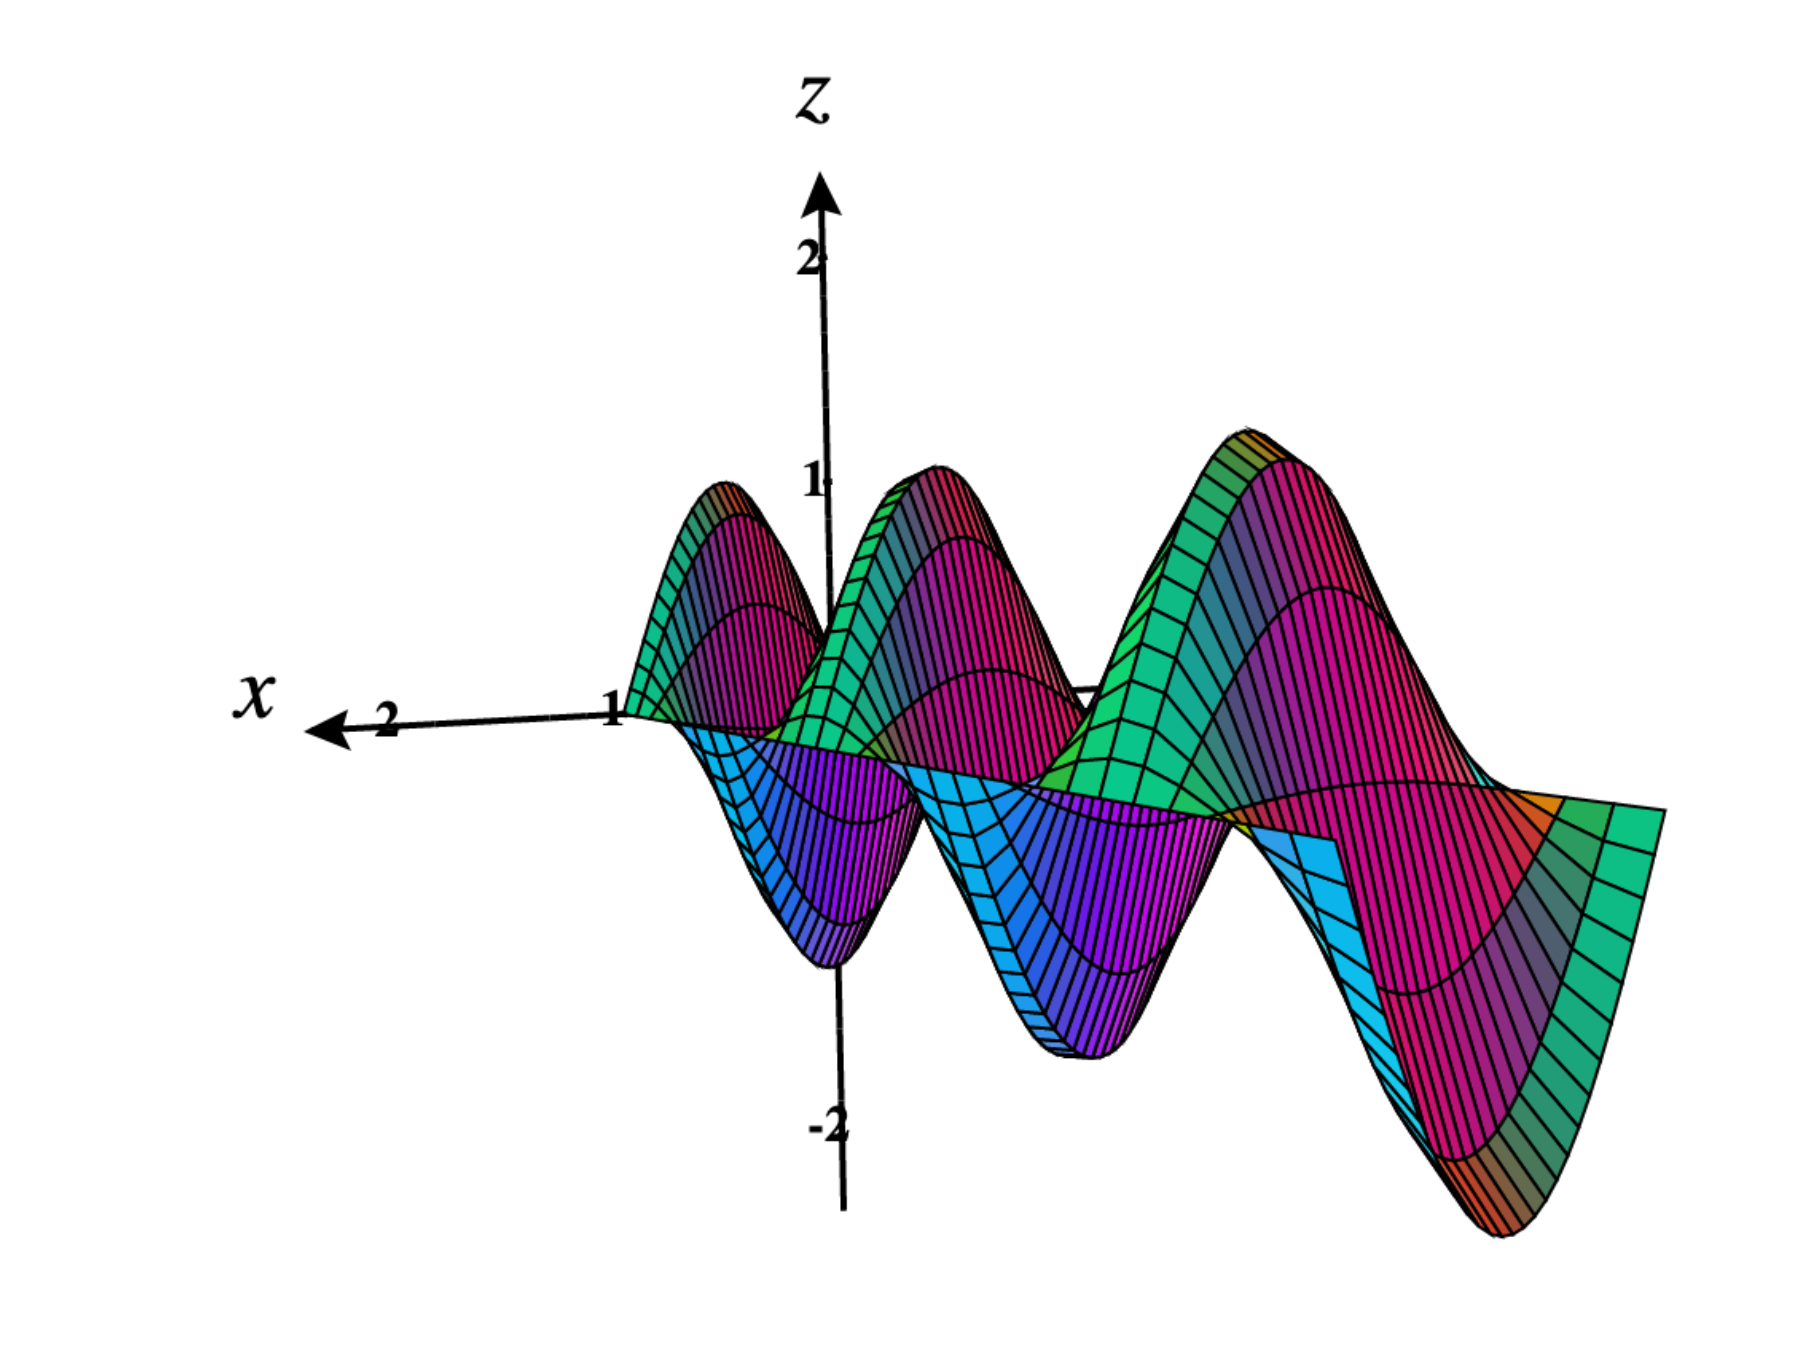
\includegraphics[width=.5\textwidth]{Figures/wave_solution.png}
        % \end{figure}
        \end{ex}

% \end{document}
